\chapter{Permutations}
Recall that permutation is a bijection from $[n]$ to $[n]$. We already discussed
several properties of them. In this chapter we will discuss some combinatorial
properties of them. We denote by $S_n$ the set of all permuations of
$[n]$.\footnote{%
  Letter $S$ is used since in the group theory this set is called
  the symmetric group.
}
\nomenclature[S]{$S_n$}{denote the set of all permuations of $[n]$}


The main operation over permutations is composition, for two permutations $p$
and $q$ we denote their composition $p \circ q$ by $pq$.\footnote{%
  Some authors dentoe $q \circ p$ by $pq$.
}
Note that this operation is not commutative; i.e. $p \circ q$ is not
necessarily equal to $q \circ p$.

Every permutation $p$ can is uniquely detemined by the values $p(1)$, \dots,
$p(n)$, thus sometimes we denote the permutation $f$ by a seqence
$p(1) p(2) \dots p(n)$ (we call it \emph{one-line notation}).
For example, the permutation $3 1 2$ is equal to the function $p : [3] \to [3]$
such that
\[
  p(x) =
  \begin{cases}
    3 & \text{if } x = 1 \\
    1 & \text{if } x = 2 \\
    2 & \text{if } x = 3
  \end{cases}.
\]


\section{Cycles}
Consider the permutation $p$ equal to $2 3 1 5 4$ and draw a digram with
$5$ points where we draw an arrow from $i$ to $j$ iff $p(i) = j$.
\begin{center}
  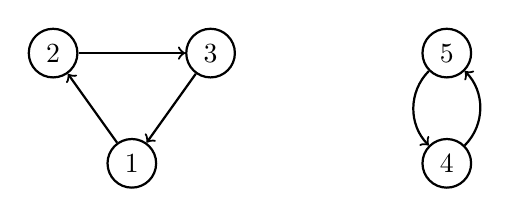
\begin{tikzpicture}[thick]%
    \node[circle, draw, minimum width=4pt]
      (p1) at (0, 0) {1};
    \node[circle, draw, minimum width=4pt]
      (p2) at (-1, 1.4) {2};
    \node[circle, draw, minimum width=4pt]
      (p3) at (1, 1.4) {3};
    \node[circle, draw, minimum width=4pt]
      (p4) at (4, 0) {4};
    \node[circle, draw, minimum width=4pt]
      (p5) at (4, 1.4) {5};
    \draw[->] (p1) -- (p2);
    \draw[->] (p2) -- (p3);
    \draw[->] (p3) -- (p1);

    \draw[->] (p4) to[out=45, in=-45] (p5);
    \draw[->] (p5) to[out=-135, in=135] (p4);
  \end{tikzpicture}
\end{center}
It is easy to see that there are two ``cycles'' in the diagram. In this section
we prove that this is not a coincedence and we also study some properties of
permutations with respect to the structure of these cycles.

\begin{definition}
  Let $p$ be a permutation of $[n]$, $x \in [n]$, and $i$ be the smallest
  integer such that
  $p^i(x) = \underbrace{p(p(\dots p(}_{i \text{ times}} x) \dots )) = x$.
  The we say that the entries $x$, $p(x)$, \dots, $p^{i - 1}(x)$ form an
  $i$-cycle in $p$.

  We denote a permuation $q : [n] \to [n]$ consisting of one cycle
  $a_1$, \dots, $a_k$ by $(a_1, \dots, a_k)$; i.e.
  \[
    q(x) =
    \begin{cases}
      a_2 & \text{if } x = a_1 \\
      a_3 & \text{if } x = a_2 \\
      \dots \\
      a_1 & \text{if } x = a_k \\
      x & \text{otherwise}
    \end{cases}.
  \]
\end{definition}

\begin{theorem}
\label{theorem:permuations-into-cycles}
  All permutations can be decomposed into the disjoint unions of their cycles.
\end{theorem}
\begin{exercise}
  Prove Theorem~\ref{theorem:permuations-into-cycles}.
\end{exercise}
For example, the discussed permuation $2 3 1 5 4$ can be decomposed into
$(1, 2, 3) (4, 5)$.

If an permutation $p : [n] \to [n]$ has $c_i$ cycles of length $i \in [n]$, then
we say that $(c_1, c_2, \dots, c_n)$ is the \emph{cycle type} of $p$.
The simplest question we may ask is ``how many permuations of a certain cyclic
type exist?'', the following theorem gives an answe for this question.
\begin{theorem}
  Let $c_1$, \dots, $c_n$ be some positive integers such that
  $\sum_{i = 1}^n i c_i = n$. Then there are
  $\frac{n!}{c_1! c_2! \dots c_n! 1^{c_1} 2^{c_2} \dots n^{c_n}}$
  permutation of the cyclic type $(c_1, \dots, c_n)$.
\end{theorem}

Note that this result allows us to answer the following problem. King Arthur has
$n$ Knights of the Round Table; Arthur wonders: how many ways to seat in the
round table? In other words he is asking how many permuations of the cyclic type
$(0, 0, \dots, 0, 1)$. Hence, the answer for Arthur's question is $n!$.

\section{Stirling Numbers of The First Kind}
In the previous chapter we defined Stirling numbers of the second kind; in this
section we define their first kind counterpart.

\begin{definition}
  Let $n > k$ be some integers. We denote the number of permutations of $[n]$
  with $k$ cycles by $c(n, k)$. The number $s(n, k) = (-1)^{n - k} c(n, k)$ is
  called a \emph{Stirling number of the first kind}.
\end{definition}
The multiplier $(-1)^{n - k}$ seems a bit strange, but we will explain it
in Theorem~\ref{theorem:connection-between-stirling-numbers}.

Like the numbers $S(n, k)$, the nunmbers $c(n, k)$ satisfy a simple reccurent
formula.
\begin{theorem}
\label{theorem:stirling-numbers-first-kind-reccurent-relation}
  Let $n \ge k$ be positive integers. Then
  \[
    c(n, k) = c(n - 1, k - 1) + (n - 1) c(n - 1, k).
  \]
\end{theorem}

\begin{exercise}
  Prove Theorem~\ref{theorem:stirling-numbers-first-kind-reccurent-relation}.
\end{exercise}

\begin{theorem}
\label{theorem:connection-between-stirling-numbers}
  For any real $x$ and positive integer $n$,
  \[
    (x)_n = \sum_{k = 0}^n s(n, k) x^k.
  \]
\end{theorem}
Now one may see why the multiplier $(-1)^{n - k}$ was necessary by comparting
this equality with the equality from
Thorem~\ref{theorem:stirling-numbers-and-polynomials} stating that
\[
  x^n = \sum_{k = 0}^n S(n, k) (x)_k.
\]
In other words, Stirling numbers of the second kind are ``inverse'' to the
Stirling numbers of the first kind.

We can interpret this result in terms of linear algebra. Consider the vector
space $\mathbb{P}_n$ of real polynomials of degree at most $n$. It is well
known that $1$, $x$, \dots, $x^n$ is the basis of this space; additionally,
it is easy to see that $1$, $(x)_1$, \dots, $(x)_n$ is also a basis. Then
the matrices $\mathcal{S}$ and $\mathcal{s}$ such that
$\mathcal{S}_{i, j} = S(i, j)$ and $\mathcal{s}_{i, j} = s(i, j)$ are
change of basis matrices between these two bases.

\section{Permutations with Restricted Cycle Structure}
One of the problem of the represntation of a permutation as a collection of
cycles is that it is not unique; e.g. $(1, 2, 3) (4, 5)$ and $(5, 4) (1, 2, 3)$
represent the same permuation. To avoid this we introduce a \emph{canonical
cycle form}, That is, each cycle will be written with its largest element first,
and the cycles will be written in increasing order of their first elements. Thus
the permutation's $2 3 1 5 4$ canonical cycle form is $(3, 2, 1) (5, 4)$.

Using this notation and the next lemma we can discover several nice properties
of permuations.
\begin{lemma}
\label{lemma:permuations-transfomration}
  Let $p : [n] \to [n]$ be a permutation written in canonical cycle notation.
  Let $\fpm(p)$ be the permutation obtained from $p$ by omitting the
  parentheses and reading the entries as a permutation in the one-line notation.
  Then $\fpm$ is a bijection from $S_n$ to $S_n$.
\end{lemma}
For example, $\fpm(2 3 1 5 4) = 32154$ and
$\fpm^{-1}(2 3 1 5 4) = (2) (3, 1) (5, 4) = (3, 1) (5, 4)$.

Using this transfomration we may prove the following result, which is very
technical without this transfomration.
\begin{theorem}
  Let $n$ be a positive integer and $i \neq j \in [n]$. There are $n! / 2$
  permuations of $[n]$ such that $i$ and $j$ are in the same cycle.
\end{theorem}
\begin{proof}
  Without loss of generality, $i = n$ and $j = n - 1$.

  Let $q = q_1 q_2 \dots q_n$ be a permutation of $n$, and let $\fpm(p) = q$,
  where $\fpm$ is the bijection from Lemma~\ref{lemma:permuations-transfomration}.
  The entries of $q$ that are larger than all entries on their left are called
  left-to-right maxima. Note that if $q$ has $\ell$ left-to-right maxima,
  then $p$ has t cycles. Also note that the rightmost left-to-right maximum of
  $q$ is the entry $n$.

  Therefore, the last cycle of $p$ starts with $n$, and the entries in that
  cycle of $q$ are precisely the entries on the right of $n$ in $q$. Therefore,
  $p$ contains $n$ and $n - 1$ in the same cycle if and only if $n - 1$ is on
  the right of $n$ in $q$. As that happens in half of all permutations, the
  proof follows.
\end{proof}

Another nice result states that for any $i \in [n]$, the probability that
$i$ is in a cycle of length $k$ does not depend on $k$ and is equal to $1 / n$.
\begin{theorem}
  Let $i \in [n]$. Then for all $k \in [n]$, there are exactly $(n - 1)!$
  permutations of $[n]$ in which the cycle containing $i$ is of length $k$.
\end{theorem}
\begin{proof}
  Again, it is sufficient to prove the statement for $i = n$. Let
  $q = q_1 q_2 \dots q_n$ be a permutation of $n$, let $\fpm(p) = q$, where
  $\fpm$ is the bijection from Lemma~\ref{lemma:permuations-transfomration},
  and let  $q_j = n$. Then the cycle $C$ containing $n$ in $p$ is of length
  $n - j + 1$ as $n$ itself starts the last cycle. So if we want $C$ to have
  length $k$, we must have $j = n + 1 - k$. However, there are clearly
  $(n - 1)!$ permutations of length $n$ that contain $n$ in a given position,
  and the proof follows.
\end{proof}

\begin{chapterendexercises}
  \exercise Find a formula for $c(n, n - 2)$.
  \exercise Prove that for any fixed $k$, the function $c(n, n - k)$ is a
    polynomial function of $n$. Find the degree of that polynomial.
  \exercise Let $p$ be a permutation of $[n]$. We associate a permutation matrix
    $M^{(p)}$ to $p$ as follows. Let $M^{(p)}_{i, j} = 1$ if $p(i) = j$, and let
    $M^{(p)}_{i, j} = 0$ otherwise. Prove that $|\det M^{(p)}| = 1$.
  \exercise Prove that if $p$ and $q$ are two permutations, then
    $M^{(p)} M^{(q)} = M^{(pq)}$.
  \exercise Prove that permutations $p$ and $p^{-1}$ are of the same cycle type
    for any permuation $p$.
  \exercise A permutation $p$ is called a nontrivial involution if
    $p^2 = 1 2 \dots n$, but $p \neq 12 \dots n$. Prove that if $n > 1$, the
    number of nontrivial involutions in $S_n$ is odd.
\end{chapterendexercises}
